\documentclass[border=10pt]{standalone}
\usepackage{pgfplots}
\pgfplotsset{compat=1.18}

\begin{document}
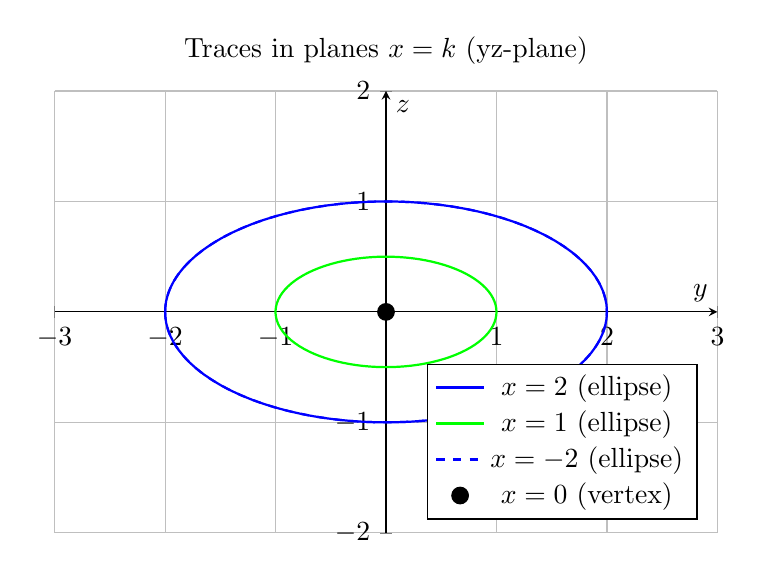
\begin{tikzpicture}
\begin{axis}[
    xlabel={$y$},
    ylabel={$z$},
    title={Traces in planes $x = k$ (yz-plane)},
    axis lines=middle,
    grid=major,
    width=10cm,
    height=8cm,
    xmin=-3, xmax=3,
    ymin=-2, ymax=2,
    axis equal image,
    legend pos=south east,
]
% Trace at x = 2: y^2 + 4z^2 = 4 (ellipse)
\addplot[domain=0:360, samples=100, thick, blue] ({2*cos(x)}, {sin(x)});
\addlegendentry{$x = 2$ (ellipse)}

% Trace at x = 1: y^2 + 4z^2 = 1 (smaller ellipse)
\addplot[domain=0:360, samples=100, thick, green] ({cos(x)}, {0.5*sin(x)});
\addlegendentry{$x = 1$ (ellipse)}

% Trace at x = -2: y^2 + 4z^2 = 4 (ellipse, shifted)
\addplot[domain=0:360, samples=100, thick, blue, dashed] ({-2*cos(x)}, {sin(x)});
\addlegendentry{$x = -2$ (ellipse)}

% Vertex at origin
\addplot[only marks, mark=*, mark size=3pt, black] coordinates {(0,0)};
\addlegendentry{$x = 0$ (vertex)}

\end{axis}
\end{tikzpicture}
\end{document}
